\chapter{Results} % Main chapter title

\label{chap:results} % For referencing the chapter elsewhere, use \ref{Chapter1} 

\section{Semantic Embeddings}
\subsection{Validation on English Data}
For \code{SIM} space, we used the English \code{WordNetEmbedding} trained on the first 15,000 frequent words and benchmark dataset vocabulary. We kept 511 first PCs by following the method in section \ref{subsec:semanticsimilaritymethod}.

The intersection of \code{SIM} space and the Common Crawl vocabulary used in \code{MIX} space resulted to 8157 words. 

The linear regression model mapping \code{SIM} to \code{MIX} produced a \code{r2} score of 0.1662.

Figure \ref{fig:EngDecorVarRatio} shows the PCA analysis of the resulting 4 semantic spaces. Table \ref{tab:engdecorrelationscores} shows the semantic ranking task results: though we have not completely dissociated each resulting semantic space with irrelevant semantic axis, a clear dominance of \association semantic signal is present in \code{ASN} space. 

\begin{table}
\centering
\begin{ThreePartTable}
    
\begin{tabularx}{\textwidth}{RRRRll}
    \multicolumn{6}{l}{\tabhead{English Semantic Space Semantic Ranking Task Results}} \\
\toprule
\tabhead{Semantic Space} & \tabhead{Vocabulary Size} & \tabhead{Dimension} & r & \tabhead{SimLex-999} & \tabhead{WS353-ASN} \\  
\midrule
\mr{2}{*}{\code{SIM}} & \mr{2}{*}{15K} & \mr{2}{*}{511} & Pearson & 0.5060 & \textbf{0.0279}\tnote{1} \\  
&  &  & Spearman & 0.4989 & \textbf{0.0193}\tnote{2}   \\  
\midrule
\mr{2}{*}{\code{MIX}} & \mr{2}{*}{2.2M} & \mr{2}{*}{300} & Pearson & 0.3946 & 0.6091 \\  
&  &  & Spearman & 0.3752 & 0.5709 \\  
\midrule
\mr{2}{*}{\code{ASN}} & \mr{4}{*}{8157} & \mr{4}{*}{300} & Pearson & 0.1953 & 0.5633 \\  
&  &  & Spearman & 0.2133 & 0.5918 \\ 

\cmidrule{1-1} \cmidrule{4-6}
\mr{2}{*}{\code{SIG}} &  &  & Pearson & 0.4929 & 0.2091 \\  
&  &  & Spearman & 0.4994 & 0.1678 \\  

\cmidrule{2-6}
\multicolumn{4}{r}{Out of Vocabulary} & 0.002 & 0.024 \\  
\midrule \midrule
\mr{2}{*}{Baseline\tnote{3}} & \mr{2}{*}{13k} & \mr{2}{*}{850} & Pearson & 0.50 & 0.32 \\  
    &  &  & Spearman & 0.52 & 0.33 \\  
\bottomrule
\end{tabularx}
\begin{tablenotes}
    \footnotesize
    \item[1] p-value=0.6626
    \item[2] p-value=0.7629
    \item[3] Baseline is reported by \cite{saediWordNetEmbeddings2018}. The 13k words are selected cue words in psycholinguistic experiments. They show the best performance among all tested models.
\end{tablenotes}
\end{ThreePartTable}
\caption[English Semantic Space Semantic Ranking Task Results]{\code{SIM} achieves almost the same performance as the baseline in \similarity benchmark, while it cancels out the 
\association score. \code{MIX} space performs well in both task-sets, with a slight preference for \association, consistent with \parencite{lapesaContrastingSyntagmaticParadigmatic2014}'s conclusion. \code{ASN} has comparable scores in \association with \code{MIX}, but still have a non-zero score in \similarity. Such is also the case for \code{SIG} compared with \code{SIM}.\label{tab:engdecorrelationscores}}
\end{table}

\begin{figure}
    \centering
    \makebox[\linewidth]{
    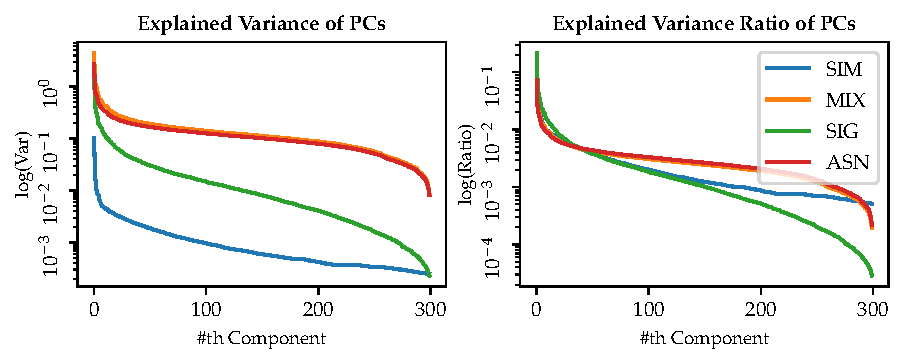
\includegraphics[scale=1]{Figures/EngDecorVarRatio.pdf}
    }
    \caption[EVR of 4 Semantic Spaces]{PCA of 4 semantic spaces of 8157 vocabulary. \textbf{Left panel}: While the variance of \code{SIM} is systematically lower than other three spaces, its projection (\code{SIG}) has larger variances. The suppression of \code{SIG} from \code{MIX} has little impact on the model's variance. \textbf{Right panel}: \code{SIG} and \code{SIM} have a denser variance concentrated on first PCs, while \code{ASN} and \code{MIX} have more homogeneous variance distributions.} 
    \label{fig:EngDecorVarRatio}
\end{figure}

\subsection{Application on French data}

Provided with the methodological success of English data, we applied the same algorithm against French data.

For \code{SIM} space, we used the French \code{WOLFEmbedding} with POS tag trained on all the available vocabulary. We kept 634 first PCs.

After rule-based and manual matching, the intersection of \code{SIM} space and the \code{MIX} space vocabulary resulted to 24519 distinct lemma with POS tags.

The linear regression model mapping \code{SIM} to \code{MIX} produced a \code{r2} score of 0.0776, which is lower than the English score, indicating a smaller informational overlap between the two embedding models.

Figure \ref{fig:FreDecorVarRatio} shows a similar PCA analysis. Though indicative, we tested the resulting semantic spaces using the same tasks against our indicative gold-standard data (section \ref{subsection:frenchbenchmarkdataconstruction}). The results (table \ref{tab:fredecorrelationscores}) puts the validity of \code{ASN} space into question: it seems to contain both \similarity and \association information.

\begin{figure}
    \centering
    \makebox[\linewidth]{
    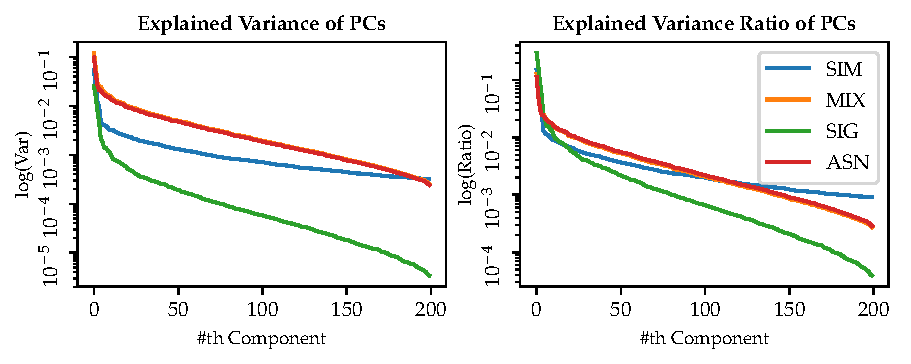
\includegraphics[scale=1]{Figures/FreDecorVarRatio.pdf}
    }
    \caption[EVR of 4 French Semantic Spaces]{PCA of 4 semantic spaces of 24519 vocabulary. \textbf{Left panel}: Due to the poor linear correlation found between \code{SIM} and \code{MIX}, the variance of \code{SIG} is systematically lower than the other three spaces, its projection (\code{SIG}) has larger variances. The suppression of \code{SIG} from \code{MIX} has also little impact on the model's variance. \textbf{Right panel}: \code{SIG} has a denser variance concentrated on first PCs, while the other three spaces have more homogeneous variance distributions.\label{fig:FreDecorVarRatio}} 
    
\end{figure}

\begin{table}
    \centering
    \begin{ThreePartTable}
    
    \begin{tabularx}{\textwidth}{RRRRll}
        \multicolumn{6}{l}{\tabhead{French Semantic Space Semantic Ranking Task Results}} \\
    \toprule
    \tabhead{Semantic Space} & \tabhead{Vocabulary Size} & \tabhead{Dimension} & r & \tabhead{SimLex-999} & \tabhead{WS353-ASN} \\  
    \midrule
    
    \mr{5}{*}{SIM} & \mr{4}{*}{56665} & \mr{4}{*}{634} & Pearson & 0.3291 & \textbf{0.1039} \\  
    &  &  & p-value & 0 & 0.1061 \\  
    \cmidrule{4-6}
    &  &  & Spearman & 0.2812 & \textbf{0.0511} \\  
    &  &  & p-value & 0 & 0.4273 \\  
    \cmidrule{2-6}

    \multicolumn{4}{r}{Out of Vocabulary} & 0.048 & 0.04 \\  
   \midrule

   \mr{4}{*}{MIX} & \mr{14}{*}{24519} & \mr{14}{*}{200} & Pearson & 0.0940 & 0.1520 \\  
   &  &  & p-value & 0.0047 & 0.0197 \\  
   \cmidrule{4-6}

    &  &  & Spearman & 0.1449 & 0.2078 \\ 
    &  &  & p-value & 0 & 0.0014 \\  

    \cmidrule{1-1} \cmidrule{4-6}

   \mr{4}{*}{ASN} &  &  & Pearson & \textbf{0.0629} & \textbf{0.1116} \\  
   &  &  & p-value & 0.0590 & 0.0879 \\  
   \cmidrule{4-6} 
    &  &  & Spearman & 0.0771 & 0.1566 \\  
    &  &  & p-value & 0.0206 & 0.0162 \\  

\cmidrule{1-1} \cmidrule{4-6}

   \mr{4}{*}{SIG} &  &  & Pearson & 0.2541 & \textbf{-0.0044} \\  
   &  &  & p-value & 0 & 0.9458 \\  
   \cmidrule{4-6}

    &  &  & Spearman & 0.3121 & \textbf{-0.0078} \\  
   &  &  & p-value & 0 & 0.9050 \\  

    \cmidrule{2-6}

    \multicolumn{4}{r}{Out of Vocabulary} & 0.0797 & 0.0711 \\  

    \bottomrule
    \end{tabularx}
    \begin{tablenotes}
        \footnotesize
        \item Scores marked in bold have a p-value larger than 0.05.
    \end{tablenotes}
    \end{ThreePartTable}
    
    \caption[French Semantic Space Semantic Ranking Task Results]{The results are consistent with English semantic spaces, despite the poor quality of French benchmark datasets. \code{SIM} has high performance in \similarity and negligible \association scores. The relatively poor de-correlation between \code{SIM} and \code{MIX} resulted a \code{ASN} still containing abundant \similarity information. \code{SIG} however, cancels out completely \association information even compared with \code{SIM} while retained \similarity signals.}
    \label{tab:fredecorrelationscores}
    \end{table}

We visualized the French semantic spaces with an embedding projector\footnote{Published as a TensorFlow component, available at \url{https://projector.tensorflow.org/}. The entries in the embedding space is presented by a sphere positioned in a 3D space, of which the coordinates are by default calculated with the first 3 PCs.} to visually control embedding quality via several exemplar lexicons and its vectorial neighbors. Based on this analysis (more details in section \ref{appsubsec:projectorvisu}), we are convinced that French \code{ASN} has a predominant \association preference.

\section{Computational Analysis of Ridge Regression}

\subsection{Regressor Generation}

\subsubsection{Vocabulary Coverage}
Each word (lexicon, lemma) in the narrated story used in fMRI experience is associated with its \code{RMS} acoustic feature temporal evolution and its semantic values in different spaces. However some of the words are not all available in our obtained spaces (table \ref{tab:lppcoverage} and \ref{apptab:lppcoverage}). When generating regressors, the semantic vectors are set to zero for out-of-vocabulary lemmas. 

\begin{table}
    \centering
    \begin{ThreePartTable}  
    \begin{tabularx}{\textwidth}{L *{10}{R}}
    \multicolumn{11}{l}{\tabhead{The Little Prince Vocabulary Coverage}} \\
    \toprule
    &  & \multicolumn{9}{l}{\tabhead{\# Instances in fMRI Recording Session}} \\
    \toprule
    \mr{2}{*}{Story} & \textbf{T} & 725 & 812 & 860 & 762 & 732 & 902 & 819 & 712 & 802 \\
    & \textbf{V} & F & 812 & 860 & 762 & 732 & 902 & 819 & 712 & 802 \\
    \midrule
    \mr{4}{*}{\parbox{0.8cm}{\code{SIM} 56665}} & TM & 36 & 30 & 32 & 27 & 30 & 33 & 24 & 30 & 27 \\
    & \% & F & 812 & 860 & 762 & 732 & 902 & 819 & 712 & 802 \\
    & VM & F & 812 & 860 & 762 & 732 & 902 & 819 & 712 & 802 \\
    & \% & F & 812 & 860 & 762 & 732 & 902 & 819 & 712 & 802 \\
    \midrule
    \mr{4}{*}{\parbox{0.8cm}{\code{ASN} /\code{MIX} /\code{SIG} 24519}} & TM & 48 & 47 & 38 & 37 & 48 & 60 & 35  & 37 & 41 \\
    & \% & F & 812 & 860 & 762 & 732 & 902 & 819 & 712 & 802 \\
    & VM & F & 812 & 860 & 762 & 732 & 902 & 819 & 712 & 802 \\
    & \% & F & 812 & 860 & 762 & 732 & 902 & 819 & 712 & 802 \\
    \bottomrule
    \end{tabularx}
    \end{ThreePartTable}
    \caption[The Little Prince Vocabulary Coverage in Semantic Spaces]{\textbf{T}: Token, \textbf{V}: Vocabulary, M: Miss\label{tab:lppcoverage}}
    \end{table}



\subsubsection{Corpus-Targeted Semantic Feature Selection}

The PCA dimension cutting methods presented in section \ref{subsec:semanticsimilaritymethod} produced 634 feature dimensions for French \code{SIM}. \code{ASN}, \code{MIX} and \code{SIG} have the same dimensionality as the original DepGloVe space. 

After have generated regressors with word onset timestamps and semantic representation vectors, the variance of resulting regressors are computed and visualized in figure \ref{fig:freSIMRegVar}, \ref{fig:freASNRegVar}, \ref{fig:freSIGRegVar} and \ref{fig:freMIXRegVar}. We selected the threshold of \(10^{-8}\), which resulted 100 informative regressors for \code{SIM} space [TODO, list of regressors in SI], and all 200 regressors generated by each of other three spaces survived the selection. 

\begin{figure}
    \centering
    \makebox[\linewidth]{
    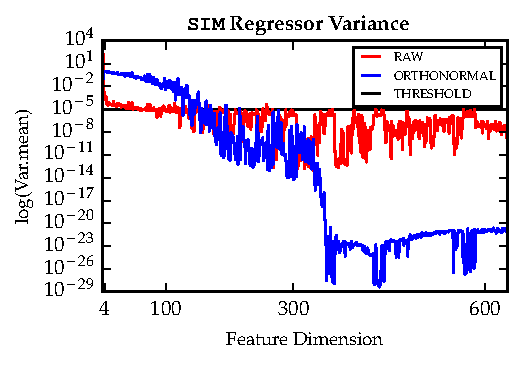
\includegraphics[scale=1]{Figures/SimDimensionSelectionRegLPP.pdf}
    }
    \caption[French \code{SIM} Regressor Variances]{Statistics on semantic regressors of 9 fMRI runs. \code{RAW} stands for regressor values directly after hemodynamic convolution, \code{ORTHONORMAL} stands for de-linearized regressors after Gram-Schmidt process. \code{THRESHOLD} is fixed at \(10^{-8}\). \textbf{Upper panel}: The minimal variance among 9 runs are shown. As \code{SIM} has a high concentration of explained variance in the first PCs (figure \ref{fig:FreDecorVarRatio}), the \code{RAW} regressors decline correspondingly for low-rank PCs. \code{ORTHONORMAL} regressors suffer more significantly and retained almost no information for the second half PCs. \textbf{Lower panel}: The average value of regressors across 9 runs shows a similar trend as the analysis on min values.} 
    \label{fig:freSIMRegVar}
\end{figure}

\begin{figure}
    \centering
    \makebox[\linewidth]{
    \includegraphics[scale=1]{Figures/ASNDimensionSelectionRegLPP.pdf}
    }
    \caption[French \code{ASN} Regressor Variances]{\code{THRESHOLD} is fixed at \(10^{-8}\). The non-PCA-transformed \code{ASN} space produced relatively more informative regressors.[TODO, figure xlabel, replace Component by dimension]} 
    \label{fig:freASNRegVar}
\end{figure}





\subsection{Impact of \(\alpha\) and Effective Feature Dimensionality}
For each of four semantic models, we generated design matrices for each fMRI session with 103 and 203 features. We sampled [TODO] \(\alpha\) and up to[TODO] feature dimension candidates by past experience, in hope of including the near-optimal hyper-parameter combination for the regression of each voxel-level model. The list of tested parameters are fixed in each model's config file\footnote{For example, \code{ASN} is configured as \url{https://github.com/nicolasying/Micipsa/blob/master/models/fr/rms-wrate-cwrate-asn200/config.json}.}, and a typical example is available in section \ref{appsubsec:alphadim}.

We selected four typical voxels in post-hoc from the regression results of run [TODO] of subject [TODO]. Each voxel is the best modeled voxel who maximizes \code{r2} among all \(\alpha\)s using only partial feature information of a certain regressor class. For example, a \code{CWRATE} class typical voxel is a voxel of which the best \code{r2} is achieved with \emph{all} first 3 features (\code{dim=3}). 

[TODO: figure Surface plot of dim/alpha]

The optimal \code{r2}s of typical voxels are never attained at the upper bound of \(\alpha\) and dimension space [TODO, refer to precedent figure]. We plotted the head-map for all voxels from session [TODO] of subject [TODO] to verify if it is also the case at the whole-brain level. In figure [TODO], each cell represents an \(\alpha\) and dimension combination. The color indicates the number of voxels having its global optimality with a given parameter set. [Todo: heat-map of dim/alpha] Since we do not have a growing trend of voxel population, this hypothesis that our parameter combination contains the near-optimal configuration for each voxel is accepted.

\section{Cognitive Analysis of fMRI Encoding}
\subsection{Basic Models}
Figure [TODO ind and group] are the whole-brain plot for regression analysis. Not that if a model overfits (i.e. \code{r2} declines) with the addition of features, the overfitted results are substituted with un-overfitted ones. Therefore, figure [TODO hist] plots the distribution of voxel-wise optimal \code{r2} (of run[], subject [] for exemplar illustration) and tracks the effective improvement when adding further feature spaces, unaffected by the overfitting problem. 

If we consider the regression model performance at each voxel as a neural activation against a potential modeled guess of local BOLD activity,
then \code{r2} activation of each individual is most of the time temporal and sometimes frontal, less often parietal even occipital. The activation peaks are found at [TODO, report peaks in table] mostly in bilateral mSTS/pSTS [TODO, ROI analysis] for all \code{RMS}, \code{RMS+WRATE} and \code{RMS+WRATE+CWRATE} models. 

With the presence of \code{RMS}, \code{WRATE} adds marginal information [TODO: Orhtonormal data on RIF]. However, \code{CWRATE} always brings significant improvements. The maximal improvement over \code{r2} by the single feature often exceeds a half of the best \code{r2} of the restricted model for precedently poorly modeled voxels. [TODO, histogram \& superposition of images]
This might be a direct implication of orthonormalization of our feature regressors.

The inter-subject variability is particularly pronounced. On averaging the \code{r2} of all 20 subjects, we are able to recover peak areas in bilateral mSTG/pSTS [TO verify]. The averaged improvement of \code{CWRATE} is located at TP, ITG, occipital and IFG[TODO verify]. 

\subsection{\emph{Similarity} Nested Model}

With \similarity semantic models, the constructed \code{SIM} features bring similarly significant improvements as \code{CWRATE}. The improvement found by \code{SIM} addition is more regular: clustered voxels in bilateral aSTS mSTS mITS, s parietotemporal, and IFG [TODO, check name]. Individuals show a lateralization preference for left hemisphere. 

[TODO, ind and group maps: r2 base, r2 full, r2 diff, F test(for ind)]


\subsubsection{First Observations on Semantic Hub}

[TODO, ROI analysis: F-test ROI, count]

\subsection{\emph{Association} Nested Model}
The addition of \code{ASN} features resulted more powerful results [TODO: powerful?] than \code{SIM}. Each voxel cluster found with \code{ASN} tends to be more extensive, [report significance regions]. [TODO, inferior parietal ]

\subsection{\emph{Similarity}/\emph{Association} Contrast}

\subsection{Full Embedding}
% \section{Behavioral Control}